\documentclass[11pt]{article}

\usepackage[margin=1in]{geometry}
\usepackage{mathpazo}
\usepackage[T1]{fontenc}
\usepackage{microtype}
\usepackage{booktabs}
\usepackage{graphicx}
\usepackage{siunitx}
\usepackage{xcolor}
\usepackage{parskip}
\usepackage{titlesec}
\usepackage{enumitem}
\usepackage{float}
\usepackage{caption}
\usepackage{subcaption}
\usepackage[colorlinks=true,
            linkcolor=blue!50!black,
            citecolor=blue!50!black,
            urlcolor=blue!50!black]{hyperref}

\sisetup{detect-weight=true,
         detect-family=true,
         group-digits=false,
         table-number-alignment=center}

% Slightly opened-up line spacing for readability.
\linespread{1.05}

% Paragraph spacing (parskip is loaded; nudge it up a touch).
\setlength{\parskip}{0.7em plus 0.2em minus 0.1em}

% Section headings: small caps, generous space above, modest below.
\titleformat{\section}
  {\normalfont\large\scshape\bfseries}{\thesection.}{0.6em}{}
\titlespacing*{\section}{0pt}{2.0ex plus 0.5ex minus 0.2ex}{0.7ex}

% No page numbers.
\pagestyle{empty}

% Avoid huge vertical glue between blocks when floats + partial pages interact.
\raggedbottom
\setlength{\textfloatsep}{10pt plus 4pt minus 3pt}
\setlength{\floatsep}{10pt plus 4pt minus 3pt}
\setlength{\intextsep}{10pt plus 4pt minus 3pt}
\captionsetup{font=small, labelfont=bf, skip=6pt, margin=0.5em}

% Tighter list separation that still breathes.
\setlist[itemize]{topsep=0.2em, itemsep=0.3em, parsep=0pt}
\setlist[enumerate]{topsep=0.2em, itemsep=0.3em, parsep=0pt}

\begin{document}

\begin{center}
{\LARGE\bfseries SLiPP++}\\[0.4em]
{\large Ten-class softmax, optimization scaffold, and BioDolphin collaboration}\\[1.1em]
{\large Filip Rumenovski}\\[0.45em]
{\normalsize \today}
\end{center}

\vspace{1em}
\noindent\rule{\textwidth}{0.4pt}
\vspace{0.85em}

SLiPP++ keeps the SLiPP data contract and the binary-collapse evaluation intact while reformulating the model as a ten-class softmax over \{ADN, B12, BGC, CLR, COA, MYR, OLA, PLM, PP, STE\}. Three of the four headline metrics improve over the Chou et al.\ 2025 baseline \cite{chou2025}; the remaining metric, apo-PDB F1, is within $-0.009$. A holdout-disciplined deployable artifact (exp-021) is selected over the higher-internal-CV artifact (exp-019) because the latter regresses on both external holdouts. The memo closes with a proposed extension to BioDolphin v1.1 \cite{yang2024} as a Dassama-lab collaboration.

\section{What SLiPP++ keeps from SLiPP}

\begin{itemize}
\item Same \texttt{training\_pockets.csv} (15{,}219 rows; ten ligand classes), sourced from \href{https://github.com/dassamalab/SLiPP_2024}{\nolinkurl{github.com/dassamalab/SLiPP_2024}}.
\item Same apo-PDB and AlphaFold supplementary holdout workbooks.
\item Same 17-descriptor paper-aligned baseline (\texttt{paper17}), reproduced as a sanity check.
\item The paper's binary-collapse evaluation is reported alongside every new ten-class metric, so Table~1 of \cite{chou2025} stays directly comparable.
\end{itemize}

\section{What SLiPP++ adds}

\begin{enumerate}
\item Ten-class softmax reformulation. Per-class F1 is reported for every experiment.
\item Richer feature stacks: \texttt{paper17\allowbreak+\allowbreak aa20\allowbreak+\allowbreak shell12\allowbreak+\allowbreak sterol\_chemistry\allowbreak+\allowbreak tunnel\_shape\allowbreak+\allowbreak derived} ($\approx\!80$--$104$ columns), in \texttt{src/slipp\_plus/feature\_builders/}.
\item Hierarchical / composite pipeline with one-vs-neighbors specialists for hard boundary classes; the STE rescue alone lifts STE F1 from $0.398$ to $0.576$.
\item Modern optimization scaffold (tested in this branch, not yet retrained on production data): multi-objective Optuna NSGA-II + Hyperband HPO, CatBoost as a fourth flat base learner, an OOF stacked meta-learner, and configuration-layer support for multiple boundary specialists.
\item Holdout discipline. The deployable artifact is selected by a holdout-weighted score: exp-019 (internal leader) regresses on both external holdouts; exp-021 (deployable) sacrifices $0.011$ internal lipid5 macro-F1 for $\sim\!0.07$ apo-PDB and $\sim\!0.09$ AlphaFold F1.
\end{enumerate}

\section{Headline results}

\begin{table}[htbp]
\centering
\renewcommand{\arraystretch}{1.05}
\begin{tabular}{@{}l S[table-format=1.3] S[table-format=1.3] S[table-format=+1.3]@{}}
\toprule
{Metric}              & {Chou et al.\ 2025} & {SLiPP++ exp-021} & {$\Delta$} \\
\midrule
Binary F1             & 0.869 & 0.902 & +0.033 \\
Binary AUROC          & 0.970 & 0.989 & +0.019 \\
AlphaFold holdout F1  & 0.643 & 0.715 & +0.072 \\
apo-PDB holdout F1    & 0.726 & 0.717 & -0.009 \\
\bottomrule
\end{tabular}
\renewcommand{\arraystretch}{1.0}
\caption{Chou et al.\ 2025 baseline \cite{chou2025} vs.\ SLiPP++ exp-021 deployable, under the original binary-collapse protocol. The apo-PDB regression is partially attributable to the smaller 117-PDB holdout in the current supplementary workbooks (vs.\ 131 in the published Table~1).}
\label{tab:headline}
\end{table}

Figure~\ref{fig:ablation} traces sequential gains in five-lipid macro-F1 along the SLiPP++ ladder from the \texttt{paper17} baseline to the exp-021 deployable.

\begin{figure}[H]
\centering
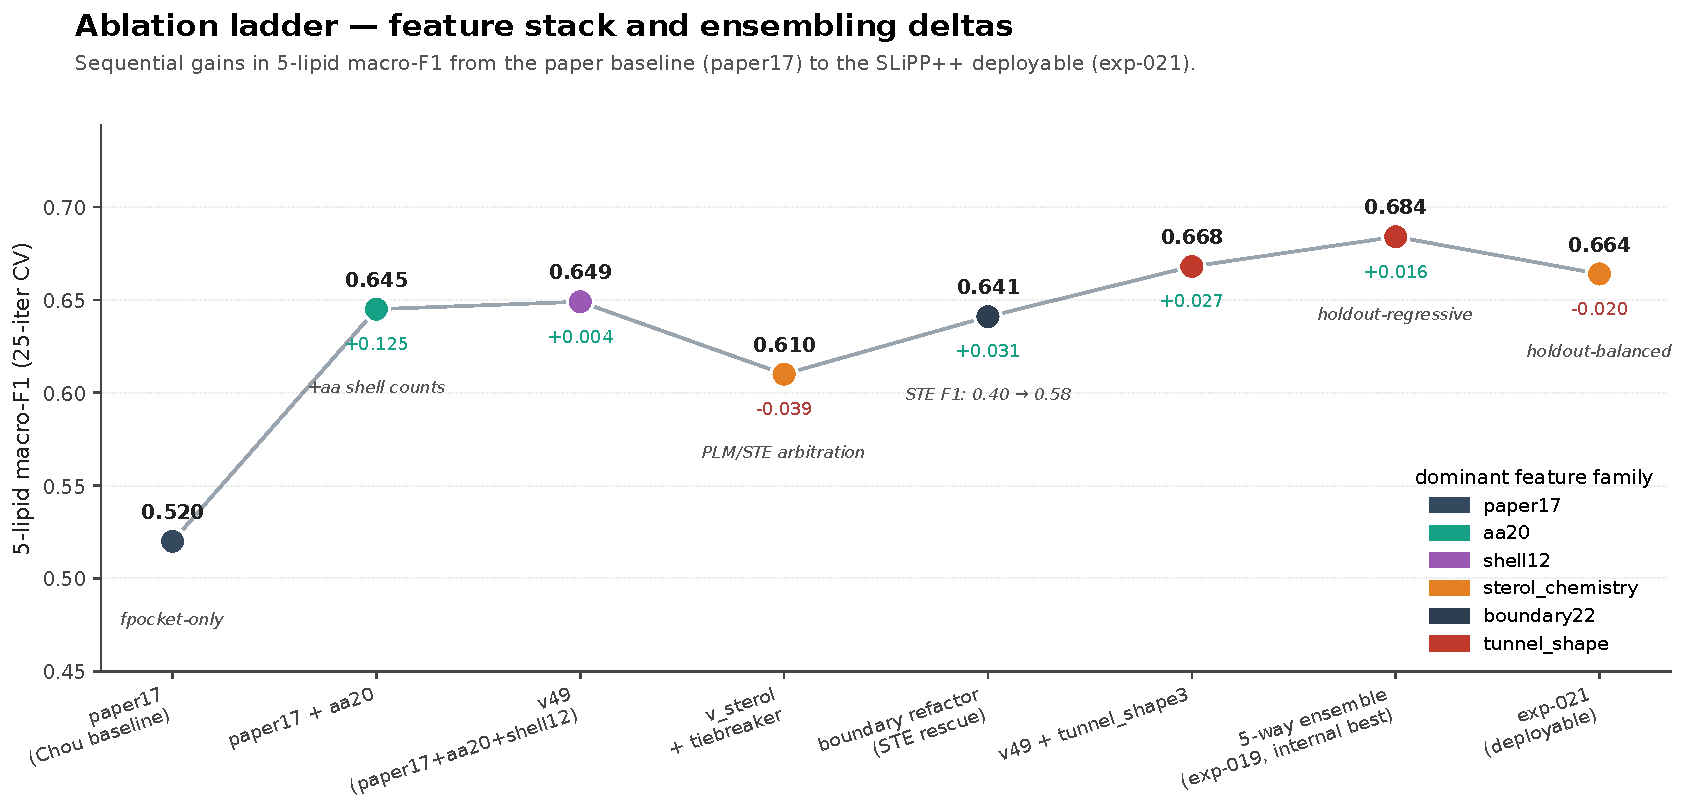
\includegraphics[width=\linewidth,height=0.74\textheight,keepaspectratio]{figures/figure_ablation_ladder.pdf}
\caption{Ablation ladder: feature-stack and ensembling milestones, with stepwise five-lipid macro-F1 from \texttt{paper17} to exp-021 (deployable). Colors encode feature family / stack identity at each rung.}
\label{fig:ablation}
\end{figure}

\section{Per-class story}

Figures~\ref{fig:landscape} and~\ref{fig:per_class} complement Figure~\ref{fig:ablation}. Figure~\ref{fig:landscape} reframes the feature analysis of \cite{chou2025} under the ten-class formulation: the hydrophobicity-dominance finding of that paper's Figure~7 is preserved, but the per-class hydrophobicity distributions and the PCA density contours show that the lipid sub-classes occupy distinct regions of pocket descriptor space. Figure~\ref{fig:per_class} shows per-class F1 for the five lipid sub-classes across the same experiment ladder; dashed vertical lines mark the Chou et al.\ paper baseline per class. Pooling lipids into a single positive class discards signal that these views recover.

\begin{figure}[H]
\centering
\captionsetup{skip=6pt}
\begin{subfigure}[t]{\linewidth}
\centering
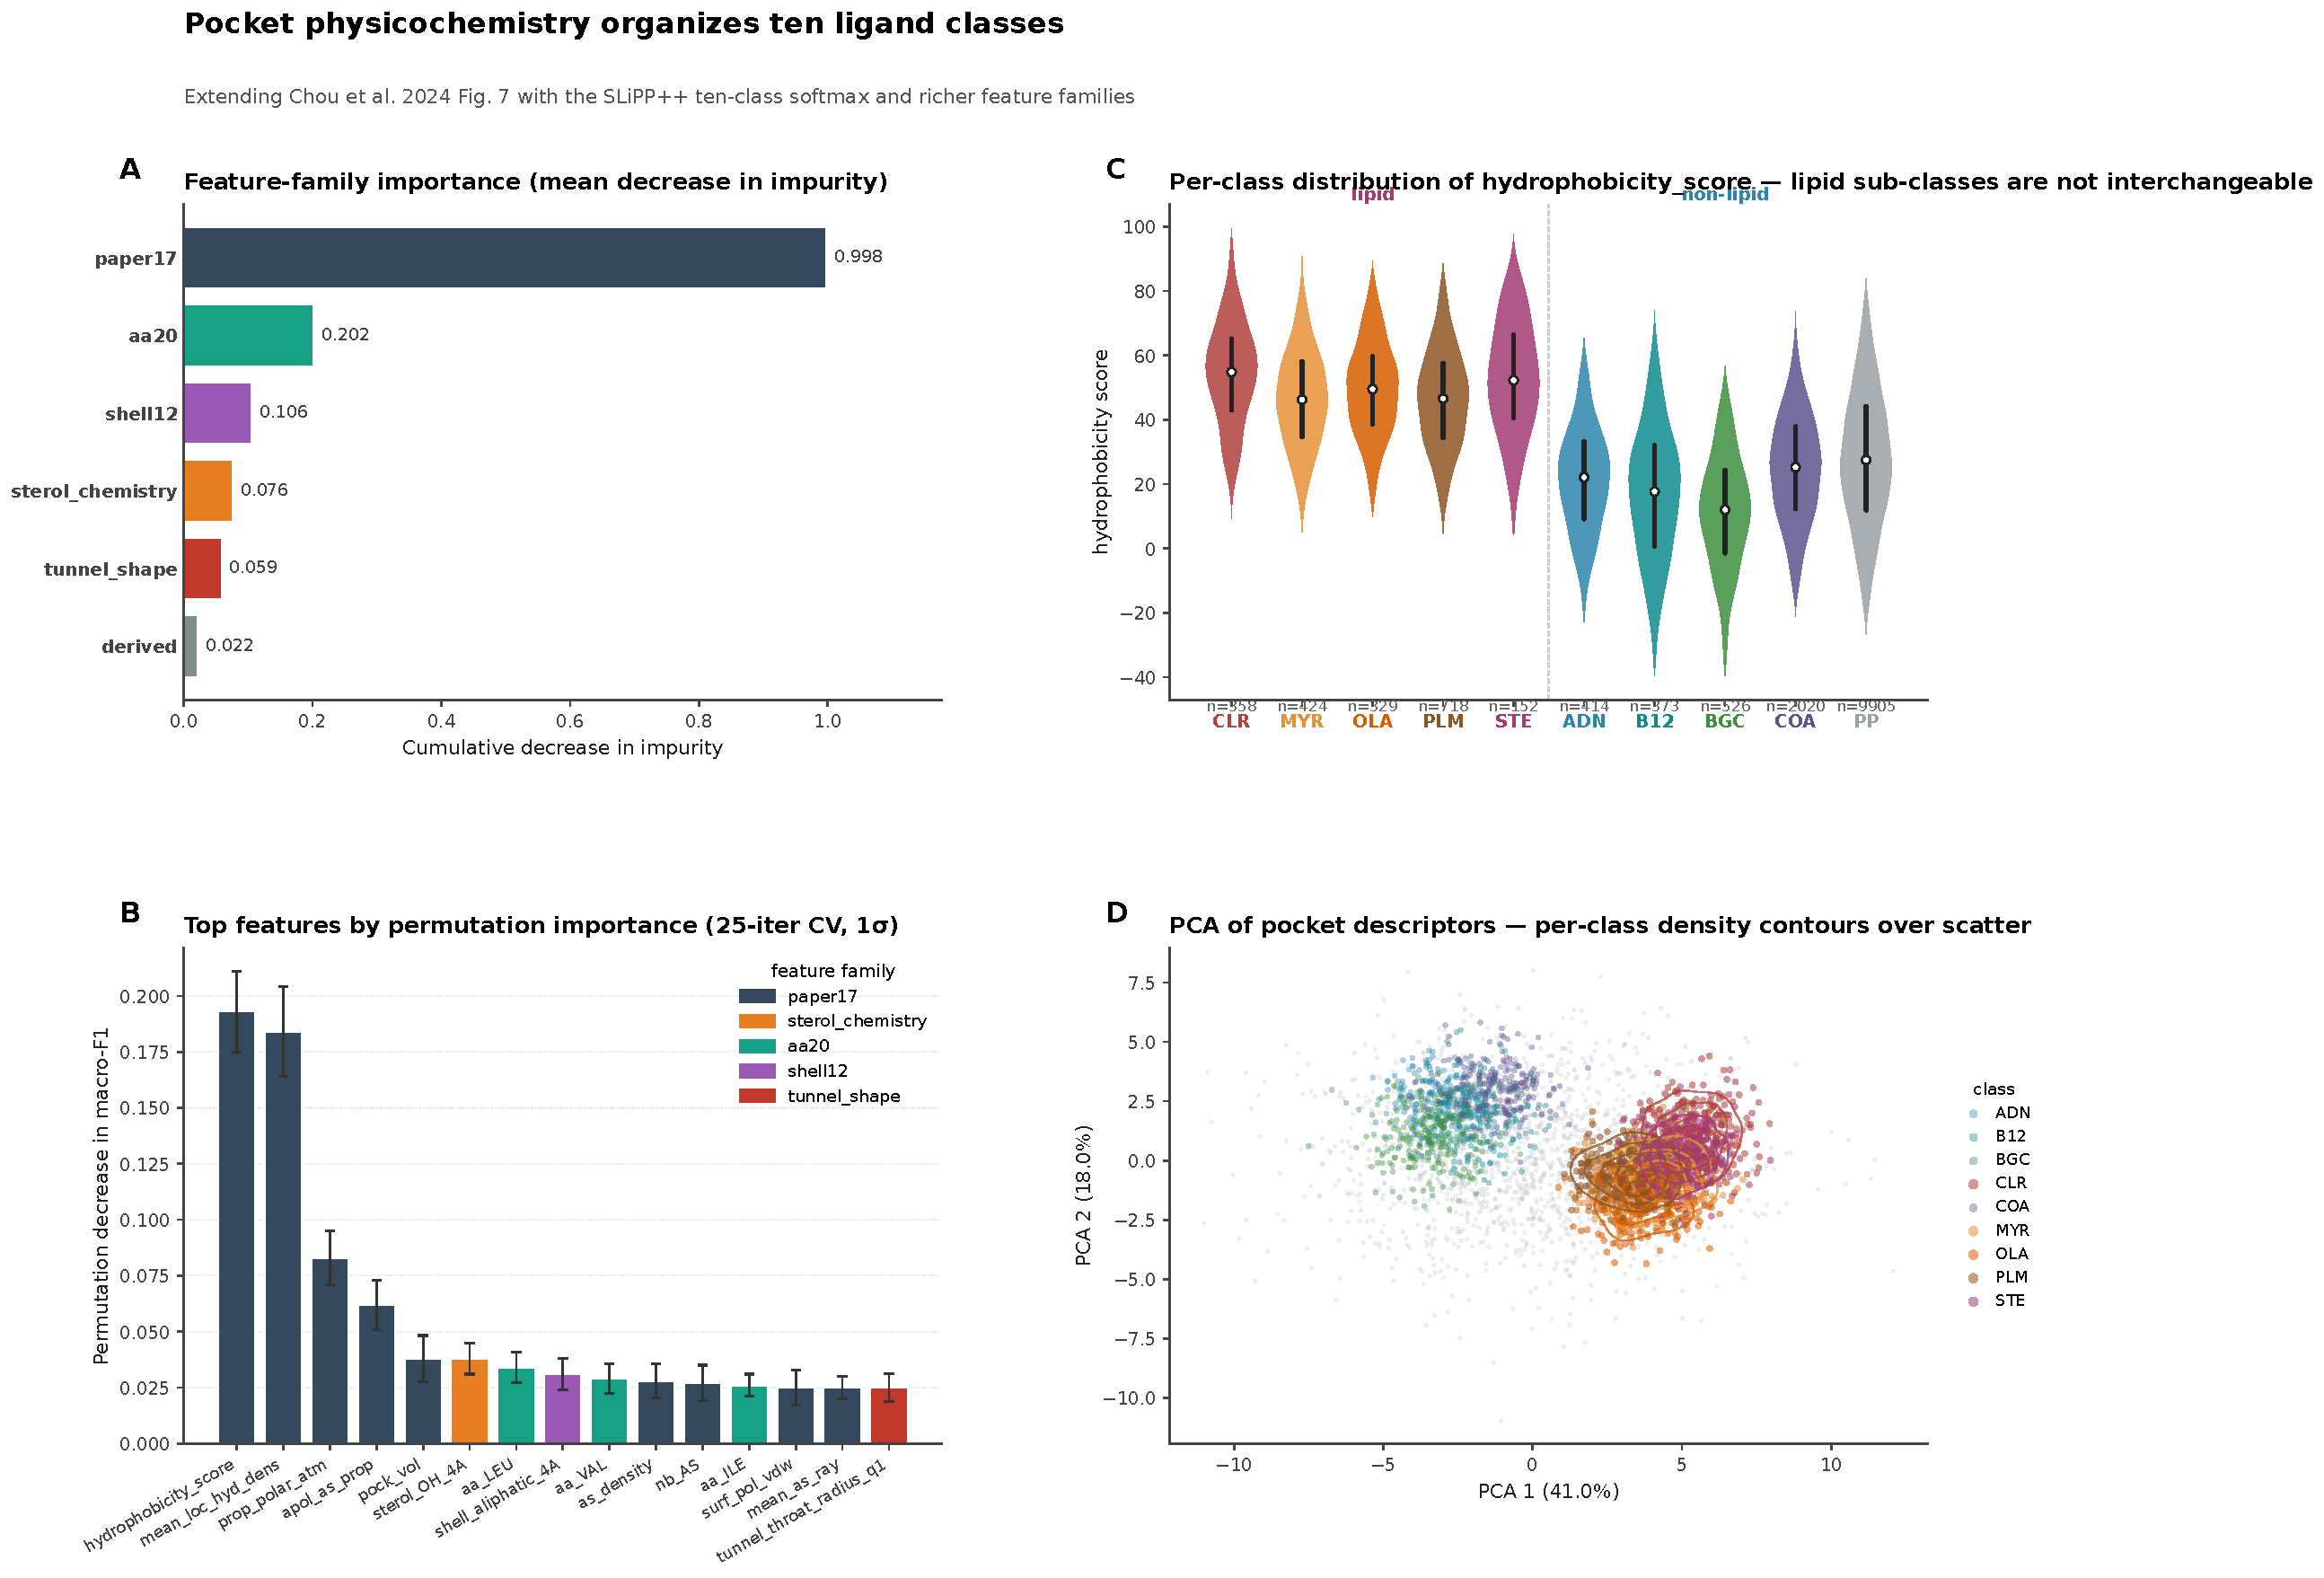
\includegraphics[width=\linewidth,height=0.42\textheight,keepaspectratio]{figures/figure7_plus_feature_landscape.pdf}
\caption{Feature landscape under the ten-class formulation. \textbf{(A)}~Feature-family importance reproduces the hydrophobicity-dominance finding of Figure~7 of \cite{chou2025} while showing that the SLiPP++ amino-acid and sterol-chemistry stacks add real signal. \textbf{(B)}~Top features by permutation F1 with $1\sigma$ error bars across 25-iteration cross-validation. \textbf{(C)}~Per-class hydrophobicity distributions across all ten classes; the lipid sub-classes are not mutually interchangeable. \textbf{(D)}~PCA with per-class density contours --- the lipid sub-classes occupy distinct regions of pocket descriptor space, supporting the ten-class formulation.}
\label{fig:landscape}
\end{subfigure}

\vspace{4pt}

\begin{subfigure}[t]{\linewidth}
\centering
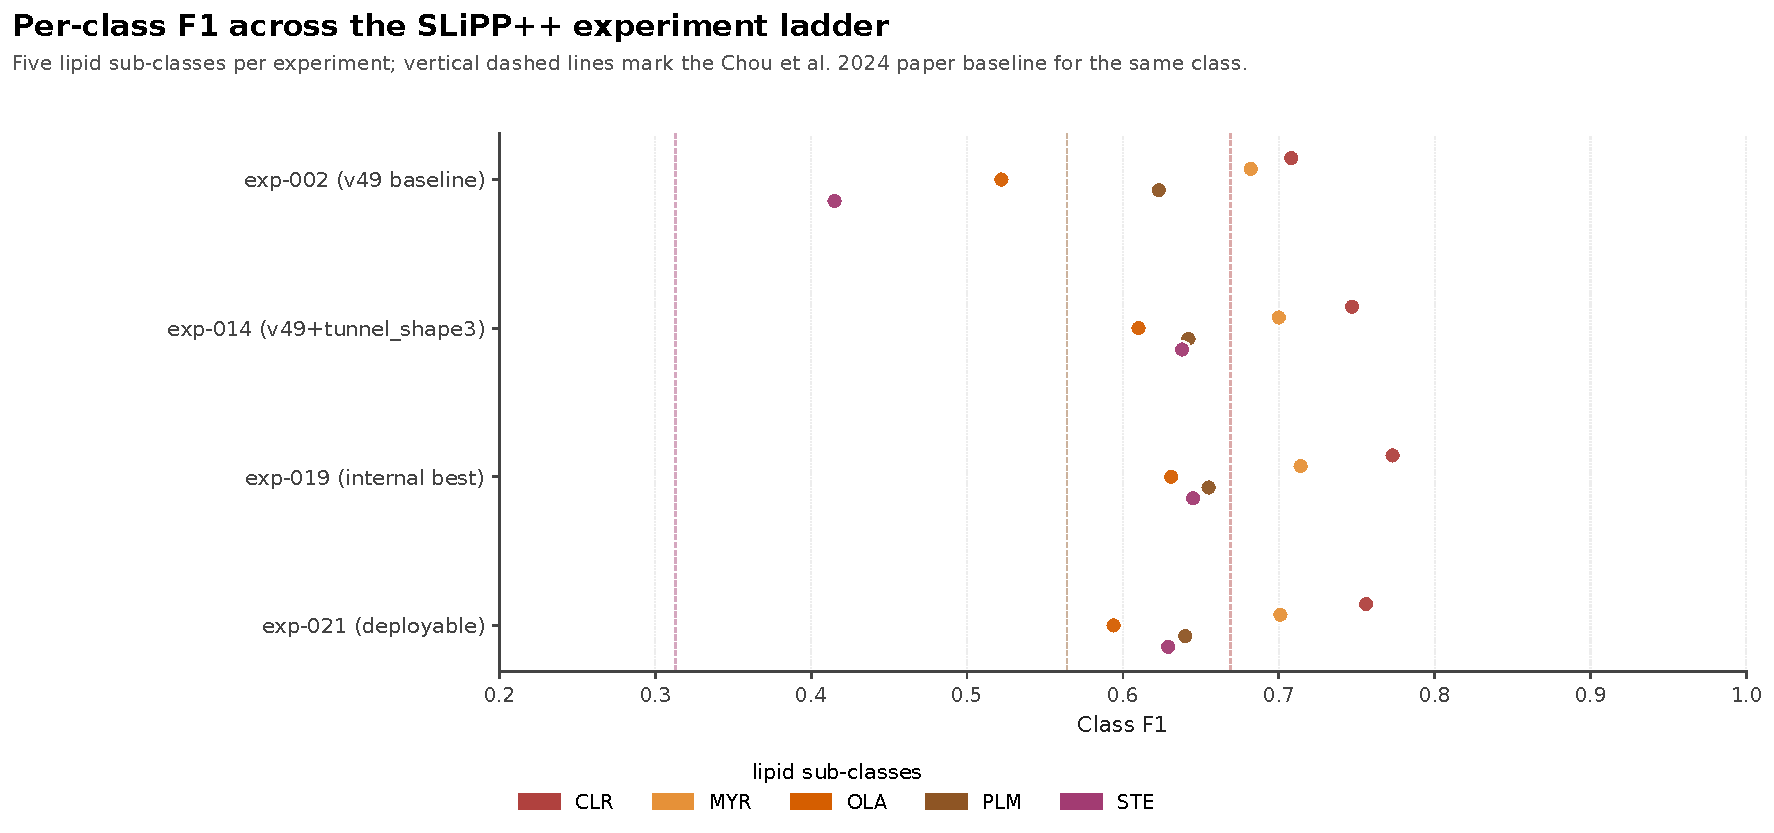
\includegraphics[width=\linewidth,height=0.30\textheight,keepaspectratio]{figures/figure_per_class_forest.pdf}
\caption{Per-class F1 (five lipid sub-classes) across the SLiPP++ experiment ladder; dashed vertical lines indicate the Chou et al.\ 2024 baseline F1 for the same class where available.}
\label{fig:per_class}
\end{subfigure}
\end{figure}

\section{Data availability and a proposed BioDolphin collaboration}

Chou et al.\ used the PDB snapshot of 27 April 2023 with a $\geq\!20$-entries-per-lipid filter, yielding 780 PDB structures and 1{,}981 lipid pockets across five lipid types \cite{chou2025}. BioDolphin v1.1 \cite{yang2024} covers 14{,}891 unique PDB structures, 127{,}359 lipid--protein interaction entries, and 2{,}619 distinct lipid molecules through 6 September 2024 --- roughly $19\times$ the structure coverage. We propose extending the SLiPP++ feature pipeline to BioDolphin v1.1 as a collaboration with the Dassama lab. The lab's lipid-class taxonomy expertise complements the SLiPP++ codebase's optimization scaffold and ten-class softmax. The full gap analysis is in \href{docs/BIODOLPHIN_EXTENSION.md}{\texttt{docs/BIODOLPHIN\_EXTENSION.md}}.

\section{Future directions}

\begin{enumerate}
\item BioDolphin v1.1 ingestion and grouped-CV retrain on the existing ten classes ($\sim\!2$ weeks, mostly compute time).
\item Optional softmax widening to include sphingolipids, phospholipids, and glycerolipids that Chou et al.\ excluded for sample-size reasons but that BioDolphin annotates at scale ($\sim\!1$ additional week).
\item Multi-objective HPO and stacking on the BioDolphin-extended dataset, now that the optimization scaffold is in place. Most of the engineering for this is already in this submission branch but has not yet been exercised on production data.
\end{enumerate}

\section{Closing}

SLiPP \cite{chou2025} is the foundation this work extends; the ten-class formulation, the optimization scaffold, and the BioDolphin pathway exist in SLiPP++ only because that foundation was laid. The SLiPP++ codebase is MIT-licensed and reproducible from a single config and lockfile, with an overview in \href{README.md}{\texttt{README.md}} and a machine-readable experiment ledger at \href{experiments/registry.yaml}{\texttt{experiments/registry.yaml}}. We would welcome the opportunity to collaborate with the Dassama lab on the BioDolphin v1.1 extension.

\vspace{0.6em}

{\small
\bibliographystyle{abbrv}
\bibliography{refs}}

\end{document}

% =====================================================================
% refs.bib stub --- paste the entries below into a sibling refs.bib file
% =====================================================================
%
% @article{chou2025,
%   author  = {Chou, Jonathan Chiu-Chun and Chatterjee, Poulami and
%              Decosto, Cassandra M. and Dassama, Laura M. K.},
%   title   = {A Machine Learning Model for the Proteome-Wide Prediction
%              of Lipid-Interacting Proteins},
%   journal = {Journal of Chemical Information and Modeling},
%   volume  = {65},
%   pages   = {9623--9638},
%   year    = {2025},
%   doi     = {10.1021/acs.jcim.5c01076}
% }
%
% @article{yang2024,
%   author  = {Yang, Li-Yen and Ping, Kaike and Luo, Yunan and
%              McShan, Andrew C.},
%   title   = {{BioDolphin} as a comprehensive database of
%              lipid--protein binding interactions},
%   journal = {Communications Chemistry},
%   volume  = {7},
%   pages   = {288},
%   year    = {2024},
%   doi     = {10.1038/s42004-024-01384-z}
% }
